\section{Relating synchronisation and linearisation}
\label{sec:relating}

In this section we describe the relationship between synchronisation
linearisation and standard linearisation.  Below, we show that the two notions
are different: synchronisation linearisation cannot, in general, be captured
directly as standard linearisation.  However, we show that synchronisation
linearisation corresponds to a small adaptation of linearisation, where one of
the operations of the synchronisation object corresponds to \emph{two}
operations of the linearisation specification object.

It is clear that standard linearisation is equivalent to synchronisation
linearisation in the (rather trivial) case that no operations synchronise, so
each operation of the synchronisation specification object corresponds to a
single operation of the concurrent object. 

We show that, given a synchronisation linearisability specification object
$SyncSpec$, it is not, in general, possible to find a linearisability
syncronisation specification $Spec$ such that for every history~$h$,\, $h$ is
synchronisation linearisable with respect to $SyncSpec$ if and only if $h$ is
linearisable with respect to $Spec$.

For example, consider the example of a synchronous channel from
Section~\ref{sec:spec}, where synchronisation linearisation is captured by
|SyncChanSpec|.  Assume (for a contradiction) that the same property can be
captured by linerisation with respect to linearisability specification~$Spec$.
Consider the history
\begin{eqnarray*}
h & = & \seq{ 
  \call.send^1(3), \call.receive^2(), 
  \return.send^1\::(), \return.receive^2()\::3 }.
\end{eqnarray*}
%
This is synchronisation linearisable with respect to |SyncChanSpec|.  By the
assumption, there must be a legal history~$h_s$ of~$Spec$ such that $h$
and~$h_s$ are compatible.  Without loss of generality, suppose the |send|
in~$h_s$ occurs before the~|receive|, i.e.
\begin{eqnarray*}
h_s & = & \seq{ send^1(3)\::(), receive^2()\::3 }.
\end{eqnarray*}
%
But the history
%
\begin{eqnarray*}
h' & = & \seq{ 
  \call.send^1(3), \return.send^1\::(), 
  \call.receive^2(), \return.receive^2()\::3 }
\end{eqnarray*}
%
is also compatible with respect to~$h_s$, so $h'$ is linearisable with respect
to~$Spec$.  But then the assumption would imply that $h'$ is synchronisation
linearisable with respect to~|SyncChanSpec|.  This is clearly false, because
the operations do not overlap.  Hence no such  linearisability
specification~$Spec$ exists.


%%%%%%%%%%%%%%%%%%%%%%%%%%%%%%%%%%%%%%%%%%%%%%%%%%%%%%%

\subsection{Two-step linearisability}

\framebox{Note: I don't think we want both this and the construction in
  Section~\ref{ssec:testing-hacking}.}

We now show that synchronisation linearisability corresponds to a small
adaptation of linearisability, but where one of the operations on the
concurrent object corresponds to \emph{two} operations of the linearisability
specification object.  We define what we mean by this, and then prove the
correspondence in the next subsection.  In the definitions below, we describe
just the differences from standard linearisation, to avoid repetition.

Given a synchronisation object with operations |op|\s1 and |op|\s2,
we will consider a linearisability specification object with signature
%
\begin{scala}
class TwoStepLinSpec{
  def op£\s1£(x£\s1£: A£\s1£): Unit
  def £$\overline{\sm{op}}_1$£(): B£\s1£
  def op£\s2£(x£\s2£: A£\s2£): B£\s2£
}
\end{scala}
%
The idea is that the operation |op|\s1 on the concurrent object will be
linearised by the composition of the two operations |op|\s1 and
$\overline{\sm{op}}_1$; but operation |op|\s2 on the concurrent object will be
linearised by just the operation |op|\s2 of the specification object, as
before.  We call such an object a \emph{two-step linearisability specification
  object}. 

We define a history~$h_s$ of such a two-step specification object much as in
Section~\ref{sec:specification-linearisability}, with the addition that for
each event $\overline{\sm{op}}_1^i()\::y$ in~$h_s$, we require that there is
an earlier event |op|$_1^i(x)\::()$ in~$h_s$ with the same invocation
identity; other than in this regard, invocation identities are not repeated
in~$h_s$.

Let $h$ be a complete concurrent history of a synchronisation object, and let
$h_s$ be a legal history of a two-step specification object corresponding to
the same invocations in the following sense:
%
\begin{itemize}
\item For every $\call.\sm{op}_1^i(x)$ and $\return.\sm{op}_1^i\::y$ in $h$,\,
  $h_s$~contains $\sm{op}_1^i(x)\::()$ and $\overline{\sm{op}}_1^i()\::y$; and
  vice versa;

\item For every $\call.\sm{op}_2^i(x)$ and $\return.\sm{op}_2^i\::y$ in $h$,\,
  $h_s$~contains $\sm{op}_2^i(x)\::y$; and vice versa.
\end{itemize}
%
We say that $h$ and $h_s$ are \emph{two-step compatible} if there is some way of
interleaving the two histories such that 
%
\begin{itemize}
\item Each $\sm{op}_1^i(x)\::()$ and $\overline{\sm{op}}_1^i()\::y$ occur
  between $\call.\sm{op}_1^i(x)$ and $\return.\sm{op}_1^i\::y$, in that
  order; 

\item Each $\sm{op}_2^i(x)\::y$ occurs between $\call.\sm{op}_2^i(x)$ and
  $\return.\sm{op}_2^i\::y$.
\end{itemize}

For example, consider a synchronous channel, with |send| corresponding
to~$op_1$, and |receive| corresponding to~$op_2$.  Then the following would be
an interleaving of two-step compatible histories of the synchronisation object
and the corresponding specification object.
\[
\seq{\begin{align} 
 \call.\sm{send}^1(3),\; \sm{send}^1(3)\::(),\; 
 \call.\sm{receive}^2(),\; \sm{receive}^2()\::3,\; \\
 \overline{\sm{send}}^1()\::(),\; \return.\sm{send}^1\::(), \;
 \return.\sm{receive}^2\::3 }.
\end{align}
\]

The definition of two-step linearisability then follows from this definition
of two-step compatability, precisely as in
Section~\ref{sec:specification-linearisability}.



%%%%%%%%%%%%%%%%%%%%%%%%%%%%%%%%%%%%%%%%%%%%%%%%%%%%%%%

\subsection{Proving the relationship}
\label{sec:twoStepLinSpec}

We now prove the relationship between synchronisation linearisation and
two-step linearisation.

Consider a synchonisation specification object |SyncSpec|.  We build a
corresponding two-step linearisation specification object~|TwoStepLinSpec|
such that synchronisation linearisation with respect to |SyncSpec| is
equivalent to two-step linearisation with respect to~|TwoStepLinSpec|.  The
definition is below: the specification's behaviour is described by the
automaton on the right.\footnote{Defining the subclasses of {\scalashape
    State} as {\scalashape case class}es allows pattern matching against such
  values.  For example, the statement {\scalashape val One(x}\s1{\scalashape )
    = state} succeeds only if {\scalashape state} has type {\scalashape One},
  and binds the name {\scalashape x}\s1 to the value of the {\scalashape x}\s1
  field of {\scalashape state}.}
\begin{trivlist}
\item[]
\begin{minipage}[b]{68mm}
\begin{scala}
trait State
case class Zero extends State
case class One(x£\s1£: A£\s1£) extends State
case class Two(y£\s1£: B£\s1£) extends State
\end{scala}
\end{minipage}
%
\hfil
%
\begin{minipage}[b]{63mm}
\begin{tikzpicture}[>= angle 60, xscale = 0.95, yscale = 0.75]
\draw (0,0) node[draw] (zero) {$\sm{Zero}$};
\draw[->] (zero) ++ (-1.5, 0) -- (zero);
%
\draw (4,0) node[draw] (one) {$\sm{One}(\sm{x}_1)$};
\draw[->] (zero)  -- node[above] {$\sm{op}_1(\sm{x}_1)$} (one); 
%
\draw (2, -2) node[draw] (two) {$\sm{Two}(\sm{y}_1)$};
\draw[->] (one)  -- node[right] {$\sm{op}_2(\sm{x}_2)$} (two); 
\draw[->] (two) -- node[left] {$\overline{\sm{op}}_1()$} (zero);
\end{tikzpicture}
\end{minipage}
%
%The specification object is defined as follows.
%
%% trait LinState
%% case class Zero extends LinState
%% case class One(x£\s1£: A£\s1£) extends LinState
%% case class Two(y£\s1£: B£\s1£) extends LinState
%
\begin{scala}
class TwoStepLinSpec{
  private var state: State = Zero
  def op£\s1£(x£\s1£: A£\s1£): Unit = {
    require(state.isInstanceOf[Zero]); state = One(x£\s1£)
  }
  def op£\s2£(x£\s2£: A£\s2£): B£\s2£ = {
    require(state.isInstanceOf[One]); val One(x£\s1£) = state
    val (y£\s1£, y£\s2£) = SyncSpec.sync(x£\s1£, x£\s2£); state = Two(y£\s1£); y£\s2£
  }
  def £$\overline{\sm{op}}_1$£(): B£\s1£ = {
    require(state.isInstanceOf[Two]); val Two(y£\s1£) = state; state = Zero; y£\s1£
  }
}
\end{scala}
\end{trivlist}
%
%
The definition forces the operations to take place in the order described by
the automaton.  In addition, the |op|\s2 operation calls the |sync| method on
|SyncSpec|, to calculate the return values and to update |SyncSpec|'s state;
it stores |op|\s1's result in the state. 

% in effect, the synchronisation happens at this point.

The following lemma follows immediately from the construction
of~|Two|\-|Step|\-|LinSpec|. 
%
\begin{lemma}
\label{lem:TwoStepLinSpec-histories}
Each history of~|TwoStepLinSpec| is the concatenation of triples of events of
the form $\sm{op}_1^{i_1}(x_1) \:: ()$,\, $\sm{op}_2^{i_2}(x_2) \:: y_2$,\,
$\overline{\sm{op}}_1^{i_1}() \:: y_1$  such that |SyncSpec| has a
corresponding legal history of events $\sm{sync}^{i_1,i_2}(x_1,x_2) \::
(y_1,y_2)$, and vice versa.
\end{lemma}

%%%%%

The following proposition reduces synchronisation linearisability to two-step
linearisability.
%
\begin{prop}
Let |SyncObj| be a synchronisation object, |SyncSpec| be a synchronisation
specification object, and let |TwoStepLinSpec| be built from |SyncSpec| as
above.  Then |SyncObj| is two-step linearisable with respect to
|Two|\-|Step|\-|LinSpec| if and only if it is synchronisation linearisable
with respect to |SyncSpec|.
\end{prop}
%%%%%%
\begin{proof}
\textbf{($\implies$).}\quad
%
Let $h$ be a concurrent history of |SyncObj|.  By assumption, there is an
extension $h'$ of~$h$, and a legal history~$h_s$ of |TwoStepLinSpec| such that
$h'' = complete(h')$ and~$h_s$ are two-step compatible.
%
Build a history~$h_s'$ of |SyncSpec| by replacing each triple
$\sm{op}_1^{i_1}(x_1) \:: ()$,\, $\sm{op}_2^{i_2}(x_2) \:: y_2$,\,
$\overline{\sm{op}}_1^{i_1}() \:: y_1$ in~$h_s$ by the event
$\sm{sync}^{i_1,i_2}(x_1,x_2) \:: (y_1,y_2)$.  
%
The history~$h_s'$ is legal by Lemma~\ref{lem:TwoStepLinSpec-histories}.  
%
It is possible to interleave $h''$ and~$h_s'$ by placing each event
$\sm{sync}^{i_1,i_2}(x_1,x_2) \:: (y_1,y_2)$ in the same place as the
corresponding event $\sm{op}_2^{i_2}(x_2) \:: y_2$ in the interleaving
of~$h''$ and~$h_s$; by construction, this is between
$\call.\sm{op}_1^{i_1}(x_1)$ and~$\return.\sm{op}_1^{i_1} \:: y_1$, and
between $\call.\sm{op}_2^{i_2}(x_2)$ and~$\return.\sm{op}_2^{i_2} \:: y_2$.
%
Hence $h''$ and~$h_s$ are synchronisation compatible, so $h''$ is
synchronisation lineariable, and so $h$ is synchronisation linearisable.

%%%%%

\textbf{($\Leftarrow$).}\quad
%
Let $h$ be a complete history of |SyncObj|.  By assumption, there is an
extension $h'$ of~$h$, and a legal history~$h_s$ of |SyncSpec| such that $h''
= complete(h')$ and~$h_s$ are synchronisation compatible.
%
Build a history~$h_s'$ of |TwoStepLinSpec| by replacing each event
$\sm{sync}^{i_1,i_2}(x_1,x_2) \:: (y_1,y_2)$ in~$h_s$ by the three events
$\sm{op}_1^{i_1}(x_1) \:: ()$,\, $\sm{op}_2^{i_2}(x_2) \:: y_2$,\,
$\overline{\sm{op}}_1^{i_1}() \:: y_1$.
%
The history~$h_s'$ is legal by Lemma~\ref{lem:TwoStepLinSpec-histories}.
%
It is possible to interleave $h''$ and~$h_s'$ by placing each triple
$\sm{op}_1^{i_1}(x_1) \:: ()$,\, $\sm{op}_2^{i_2}(x_2) \:: y_2$,\,
$\overline{\sm{op}}_1^{i_1}() \:: y_1$ in the same place as the corresponding
event $\sm{sync}^{i_1,i_2}(x_1,x_2) \:: (y_1,y_2)$ in the interleaving
of~$h''$ and~$h_s$; by construction, each $\sm{op}_1^{i_1}(x_1) \:: ()$ and
$\overline{\sm{op}}_1^{i_1}() \:: y_1$ are between
$\call.\sm{op}_1^{i_1}(x_1)$ and~$\return.\sm{op}_1^{i_1} \:: y_1$; and each
$\sm{op}_2^{i_2}(x_2) \:: y_2$ is between $\call.\sm{op}_2^{i_2}(x_2)$
and~$\return.\sm{op}_2^{i_2} \:: y_2$.
%
Hence $h''$ and~$h_s$ are two-step compatible, so $h''$ is two-step
lineariable, and so $h$ is two-step linearisable.
\end{proof}

%%%%%%%%%%

The two-step linearisation specification object can often be significantly
simplified from the template definition above.  Here is such a specification
object for a synchronous channel.
%
\begin{scala}
object SyncChanTwoStepLinSpec{
  private var state = 0        // Takes values 0, 1, 2, cyclically 
  private var value: A = _    // The current value being sent
  def send(x: A): Unit = { require(state == 0); value = x; state = 1 }
  def receive(u: Unit): A = { require(state == 1); state = 2; value }
  def £$\overline{\sm{send}}$£(): Unit = { require(state == 2); state = 0 }
}
\end{scala}

%%%%%%%%%%%%%%%%%%%%%%%%%%%%%%%%%%%%%%%%%%%%%%%%%%%%%%%

\subsection{Variations}
\label{ssec:relating-variations}

The results of this section carry across to non-binary synchronisations, in a
straightforward way.  For a synchronisation object with $k$ operations,
|op|\s1, \ldots, |op|$_k$, the operations |op|\s1, \ldots, |op|$_{k-1}$ are
each linearised in two steps.  The two-step linearisation specification object
has $2k-1$ operations, |op|\s1, \ldots, |op|$_k$, $\overline{\sm{op}}_1$,
\ldots, $\overline{\sm{op}}_{k-1}$.  The specification object encodes an
automaton with $2k-1$ states.  The figure below gives the automaton in the
case $k = 4$.
%
\begin{center}
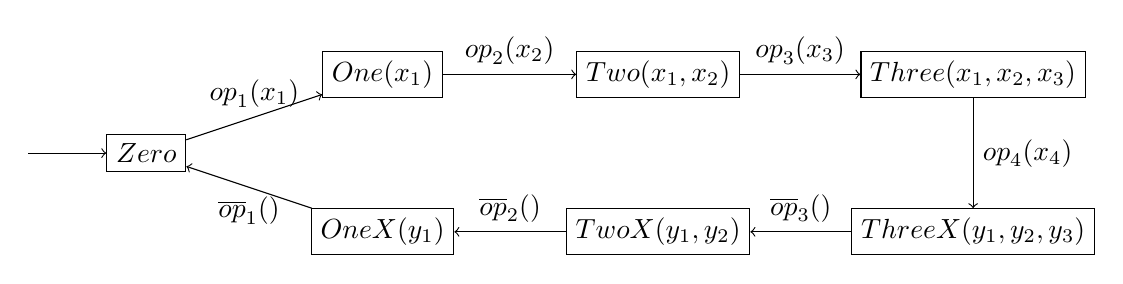
\begin{tikzpicture}[xscale = 1]
\draw (0,0) node[draw] (zero) {$\sm{Zero}$};
\draw[->] (zero) ++ (-1.5, 0) -- (zero);
%
\draw (zero)++(3,1) node[draw] (one) {$\sm{One}(\sm{x}_1)$};
\draw[->] (zero)  -- node[above] {$\sm{op}_1(\sm{x}_1)$} (one); 
%
\draw (one)++(3.5, 0) node[draw] (two) {$\sm{Two}(\sm{x}_1, \sm{x}_2)$};
\draw[->] (one)  -- node[above] {$\sm{op}_2(\sm{x}_2)$} (two); 
%
\draw (two)++(4, 0) node[draw] (three) 
  {$\sm{Three}(\sm{x}_1, \sm{x}_2, \sm{x}_3)$};
\draw[->] (two)  -- node[above] {$\sm{op}_3(\sm{x}_3)$} (three); 
%
\draw (three)++(0,-2) node[draw] (threeX) 
  {$\sm{ThreeX}(\sm{y}_1, \sm{y}_2, \sm{y}_3)$};
\draw[->] (three)  -- node[right] {$\sm{op}_4(\sm{x}_4)$} (threeX); 
%
\draw (threeX)++(-4,0) node[draw] (twoX) {$\sm{TwoX}(\sm{y}_1, \sm{y}_2)$};
\draw[->] (threeX)  -- node[above] {$\overline{\sm{op}}_3()$} (twoX); 
%
\draw (twoX)++(-3.5,0) node[draw] (oneX) {$\sm{OneX}(\sm{y}_1)$};
\draw[->] (twoX)  -- node[above] {$\overline{\sm{op}}_2()$} (oneX);
\draw [->] (oneX)  -- node[below] {$\overline{\sm{op}}_1()$} (zero);
\end{tikzpicture}
\end{center}
%
The middle operation, |op|\s4 in the above figure, applies the |sync| method
of the synchronisation specification object to the parameters $\sm x_1,
\ldots, \sm x_k$ to obtain the results $\sm y_1, \ldots, \sm y_k$; it
stores the first $k-1$ in the state, and returns $\sm y_k$. 
